\begin{figure}%[H]
	\begin{center}
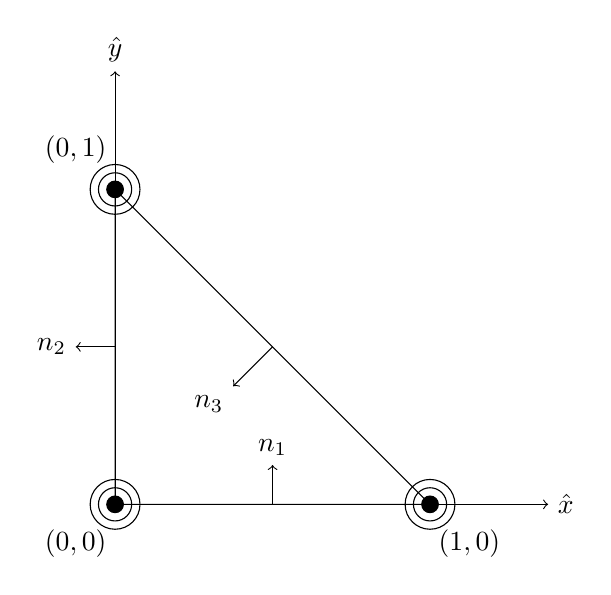
\begin{tikzpicture}
  %draw the axes
  \draw[->] (0,0) -- (5.5,0) node[right,fill=none] {$\hat{x}$};
  \draw[->] (0,0) -- (0,5.5) node[above,fill=none] {$\hat{y}$};
  %draw the triangle
	\draw (0,0) -- (4,0) -- (0,4) -- cycle;
	%draw the interpolation points
	%function values
	\filldraw (0,0) circle(3pt);
	\filldraw (4,0) circle(3pt);
	\filldraw (0,4) circle(3pt);
	%first derivatives
	\draw (0,0) circle(6pt);
	\draw (4,0) circle(6pt);
	\draw (0,4) circle(6pt);
	%second derivatives
	\draw (0,0) circle(9pt);
	\draw (4,0) circle(9pt);
	\draw (0,4) circle(9pt);
	%normal derivatives
  \draw[->] (2,0) -- (2,0.5) node[above,fill=none] {$n_1$};
  \draw[->] (0,2) -- (-0.5,2) node[left,fill=none] {$n_2$};
  \draw[->] (2,2) -- (1.5,1.5) node[below left,fill=none] {$n_3$};
  %label vertices
  %\node[circle] at (-0.6,0) {$1$};
  %\node at (4,-0.6) {$2$};
  %\node at (-0.6,4) {$3$};
  \node at (-0.5,-0.5) {$(0,0)$};
  \node at (4.5,-0.5) {$(1,0)$};
  \node at (-0.5,4.5) {$(0,1)$};
\end{tikzpicture}
	\end{center}
  \caption{The reference triangle $\hat{K}$ for Argyris}
	\label{fig:RefTriangle}
\end{figure}
